\section{密度的运算规则}
\label{sec:density-rules}

有了密度以后，最常用的操作是“换参考测度”：同一个函数对目标测度的积分，改写成对参考测度的加权积分；几个测度相对于同一参考的密度相加；或者经过一个中间测度连续换两次参考。本节依次建立这些规则，并对每条规则注明所需的测度关系，以及等式在哪个测度的几乎处处意义下成立。

\subsection{换测度公式}
\label{sec:density-change-of-measure}

密度的定义\eqref{eq:density-definition}只说明示性函数$\mathbf 1_A$对$\nu$的积分等于$\mathbf 1_Ah$对$\mu$的积分。积分的构造本来就是从示性函数出发，经简单函数和单调逼近推广到一般函数的，所以这个等式可以沿同一条路线推广。

\begin{theorem}[换测度公式]
\label{thm:density-change-of-measure}
设$\mu,\nu$是$(X,\mathcal A)$上的非负测度，$h$是$\nu$相对于$\mu$的密度。约定$0\cdot(+\infty)=0$。
\begin{enumerate}
 \item 对每个可测函数$f:X\to[0,+\infty]$，
 \[
  \int_Xf\,\mathrm d\nu=\int_Xfh\,\mathrm d\mu .
 \]
 \item 对实值或复值可测函数$f$，$f$对$\nu$可积当且仅当$fh$对$\mu$可积，此时上式仍成立。
\end{enumerate}
\end{theorem}

\begin{proof}
(1) 对$f=\mathbf 1_A$，左边是$\nu(A)$，右边是$\int_Ah\,\mathrm d\mu$，二者由密度的定义相等。对非负简单函数$f=\sum_ic_i\mathbf 1_{A_i}$，两边对$f$都是线性的（非负积分的线性性），所以等式成立。对一般非负可测$f$，取非负简单函数列$s_n\uparrow f$（引理~\ref{lem:integral-simple-approx}）。因$h\ge0$，$s_nh$也单调递增并逐点收敛到$fh$。对两边分别用单调收敛定理，
\[
 \int_Xf\,\mathrm d\nu=\lim_{n\to\infty}\int_Xs_n\,\mathrm d\nu=\lim_{n\to\infty}\int_Xs_nh\,\mathrm d\mu=\int_Xfh\,\mathrm d\mu .
\]
两边允许同时为$+\infty$。

(2) 对$|f|$用(1)，得$\int_X|f|\,\mathrm d\nu=\int_X|f|h\,\mathrm d\mu=\int_X|fh|\,\mathrm d\mu$，所以两种可积性等价。设$f$实值且可积，则$(fh)^\pm=f^\pm h$，对$f^+$与$f^-$分别用(1)，两边各得两个有限数，相减即得等式。复值时对实部和虚部分别使用实值情形。
\end{proof}

\term{换测度公式}（change-of-measure formula）把“对目标测度累计”改写成“对参考测度加权累计”。例如$[0,1]$上$\nu$相对于长度的密度为$h(x)=2x$，取$f(x)=x$，则
\[
 \int_{[0,1]}f\,\mathrm d\nu=\int_0^1x\cdot2x\,\mathrm dx=\frac23 .
\]
若$\nu$是概率测度，这就是用概率密度计算期望的公式。证明中没有用到任何有限性条件：只要密度存在，换测度公式就成立。

\paragraph{与推前换元的区别}
第~\ref{sec:integral-change-of-variables}节的推前公式（定理~\ref{thm:integral-pushforward-change}）
\[
 \int_Yg\,\mathrm d(T_\#\mu)=\int_Xg\circ T\,\mathrm d\mu
\]
也是一种“换测度”，但它改变的是所在空间：点经映射$T$从$X$搬到$Y$，被积函数相应地复合上$T$。换测度公式则留在同一空间$X$上，点不移动，被积函数不变，只是每一处的权重乘上$h$。两种操作可以接连使用：若推前测度$T_\#\mu$有相对于参考测度的密度$q$，那么先推前再换测度，就把$X$上的积分化为$Y$上的加权积分$\int_Ygq\,\mathrm d\lambda$。第~\ref{sec:density-pushforward}小节正是这样计算推前测度的密度。

\subsection{密度的线性组合}
\label{sec:density-linear}

\paragraph{共同参考测度下的加法}
设$\nu_1,\dots,\nu_m$相对于同一个参考测度$\mu$分别有密度$h_1,\dots,h_m$，$a_1,\dots,a_m\ge0$。由非负积分的线性性，对每个可测集$A$，
\[
 \sum_{i=1}^ma_i\nu_i(A)=\sum_{i=1}^ma_i\int_Ah_i\,\mathrm d\mu=\int_A\sum_{i=1}^ma_ih_i\,\mathrm d\mu,
\]
所以$\sum_ia_i\nu_i$的密度是$\sum_ia_ih_i$。这里关键是参考测度相同：密度是相对于参考的换算比例，只有同一种参考下的比例才能直接相加，正如以不同货币计价的价格不能直接相加。

\paragraph{差与有限性}
对差的处理要谨慎。若$\nu_1,\nu_2$是有限测度，则$h_1,h_2$可积，$\eta=a\nu_1-b\nu_2$（$a,b$为实数）是有限有符号测度，由可积函数积分的线性性，它的密度是可积函数$ah_1-bh_2$，与定理~\ref{thm:density-signed}一致。对无限测度不能这样做：在$\mathbb R$上取$\nu_1=\nu_2=\lambda$，形式上$h_1-h_2=0$，可$\nu_1(\mathbb R)-\nu_2(\mathbb R)=\infty-\infty$没有定义，所以“$\nu_1-\nu_2$”根本不是一个在所有集合上都有值的对象，不能仅凭密度相减就宣称它的密度为$0$。

\paragraph{混合测度的统一表示}
共同参考测度也能用来表示一个相对于长度没有密度的测度。在$[0,1]$上取参考测度$\mu=\lambda|_{[0,1]}+\delta_0$。先计算两个分量相对于$\mu$的密度。对可测集$A\subseteq[0,1]$，
\[
 \begin{aligned}
  \int_A\mathbf 1_{(0,1]}\,\mathrm d\mu&=\lambda(A\cap(0,1])+\delta_0(A\cap(0,1])=\lambda(A),\\
  \int_A\mathbf 1_{\{0\}}\,\mathrm d\mu&=\lambda(A\cap\{0\})+\delta_0(A\cap\{0\})=\delta_0(A),
 \end{aligned}
\]
其中第一式用了$\lambda(\{0\})=0$与$0\notin(0,1]$，第二式用了$\lambda(\{0\})=0$。所以$\mathrm d\lambda|_{[0,1]}/\mathrm d\mu=\mathbf 1_{(0,1]}$，$\mathrm d\delta_0/\mathrm d\mu=\mathbf 1_{\{0\}}$。由线性组合规则，$a,b\ge0$时
\[
 \nu=a\lambda|_{[0,1]}+b\delta_0,\qquad \frac{\mathrm d\nu}{\mathrm d\mu}=a\mathbf 1_{(0,1]}+b\mathbf 1_{\{0\}},
\]
总质量$\nu([0,1])=a+b$。当$b>0$时$\nu$在长度零测集$\{0\}$上有正质量，整体没有Lebesgue密度；换用共同参考$\mu$后，点质量与长度质量就能由一个函数统一表示。图~\ref{fig:density-mixed-reference}取$a=3/4$、$b=1/4$。

\begin{figure}[!htbp]
  \centering
  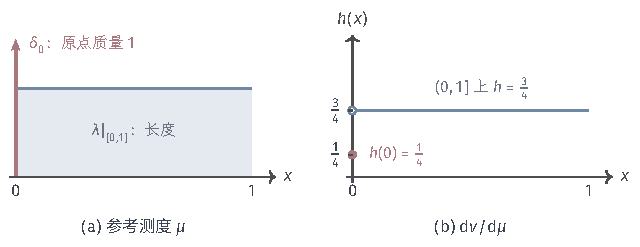
\includegraphics[width=108.433mm]{figures/02-abstract-mathematics/01-metric-and-measure/tikz/c4-mixed-reference/figure.pdf}
  \caption{在共同参考测度下统一表示混合测度。(a)参考测度$\mu=\lambda|_{[0,1]}+\delta_0$由区间上的长度（蓝色）和原点的单位点质量（红色箭头）组成。(b)$\nu=\tfrac34\lambda|_{[0,1]}+\tfrac14\delta_0$相对于$\mu$的密度：在$(0,1]$上取$3/4$，在原点取$1/4$（红色实心点）；原点处的值有意义，因为原点在$\mu$下有正质量。}
  \label{fig:density-mixed-reference}
\end{figure}

图中原点处的密度值$1/4$不能随意改动：原点在$\mu$下质量为$1$，不是$\mu$零测集。这与第~\ref{sec:density-ae-version}小节的长度参考不同，那里单点上的取值可以任意改变。哪些点上的取值有意义，取决于参考测度在那里有没有质量。

\subsection{密度的链式规则}
\label{sec:density-chain-rule}

换算比例可以连乘：先从一种参考换到中间测度，再从中间测度换到目标。为避免与Lebesgue测度的记号冲突，本小节用$\rho$表示最底层的参考测度。

\begin{theorem}[密度的链式规则]
\label{thm:density-chain-rule}
设$\rho,\mu,\nu$是$(X,\mathcal A)$上的$\sigma$有限非负测度，且$\nu\ll\mu\ll\rho$。则$\nu\ll\rho$，并且
\[
 \frac{\mathrm d\nu}{\mathrm d\rho}=\frac{\mathrm d\nu}{\mathrm d\mu}\cdot\frac{\mathrm d\mu}{\mathrm d\rho}\qquad\rho\text{-几乎处处}.
\]
\end{theorem}

\begin{proof}
由Radon–Nikodym定理，取$g=\mathrm d\nu/\mathrm d\mu$与$k=\mathrm d\mu/\mathrm d\rho$。对任意可测集$A$，先用$g$的定义，再对非负函数$\mathbf 1_Ag$与密度$k$使用换测度公式，
\[
 \nu(A)=\int_X\mathbf 1_Ag\,\mathrm d\mu=\int_X\mathbf 1_Agk\,\mathrm d\rho=\int_Agk\,\mathrm d\rho .
\]
所以$gk$是$\nu$相对于$\rho$的一个密度，由定理~\ref{thm:density-weighted-measure}得$\nu\ll\rho$。$\nu,\rho$都$\sigma$有限，由Radon–Nikodym定理中的唯一性，任何版本的$\mathrm d\nu/\mathrm d\rho$都与$gk$ $\rho$-几乎处处相等。
\end{proof}

这条规则称为\term{密度的链式规则}（chain rule for densities），它与一元微积分的链式法则形式相似，但依据是集合质量的连续换算，而不是对坐标求导。图~\ref{fig:density-chain-rule}给出一个数值例子。在$[0,1]$上取$\rho=\lambda|_{[0,1]}$，$\mathrm d\mu/\mathrm d\rho=2x$，$\mathrm d\nu/\mathrm d\mu=\tfrac32x$。链式规则给出$\mathrm d\nu/\mathrm d\lambda=3x^2$。可以直接核对：$\mu([0,1])=\int_0^12x\,\mathrm dx=1$，$\nu([0,1])=\int_0^1\tfrac32x\cdot2x\,\mathrm dx=\int_0^13x^2\,\mathrm dx=1$，两种算法在每个区间上都给出相同的值。

\begin{figure}[!htbp]
  \centering
  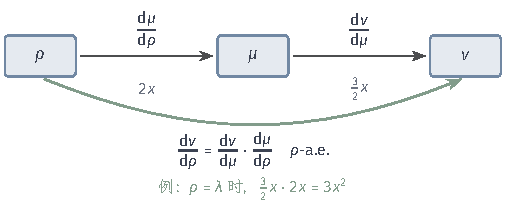
\includegraphics[width=85.651mm]{figures/02-abstract-mathematics/01-metric-and-measure/tikz/c4-chain-rule/figure.pdf}
  \caption{密度的链式规则。箭头表示“箭头终点的测度相对于起点测度的密度”：先从$\rho$换到$\mu$，再从$\mu$换到$\nu$，两段密度相乘就是从$\rho$直接换到$\nu$的密度（绿色弧线），等式在$\rho$-几乎处处意义下成立。箭头下方是$[0,1]$上$\rho=\lambda$时的例子，$2x$与$\tfrac32x$相乘得到$3x^2$。}
  \label{fig:density-chain-rule}
\end{figure}

\paragraph{版本的选择}
$g=\mathrm d\nu/\mathrm d\mu$只确定到$\mu$零测集，而结论是关于$\rho$零测集的。两者并不冲突。设$g'$是$g$的另一个版本，$g\ne g'$只发生在某个$\mu$零测集$M$上。乘积$gk$与$g'k$只可能在$M\cap\{k>0\}$上不同。由$0=\mu(M)=\int_Mk\,\mathrm d\rho$，$k$在$M$上$\rho$-几乎处处为零，所以$\rho(M\cap\{k>0\})=0$。也就是说，在$k=0$处乘积按约定取$0$，与$g$的取值无关；在$k>0$处，$\mu$的零测例外也是$\rho$的零测例外。所以无论选哪个版本，乘积都给出同一个$\rho$-几乎处处确定的密度。

\subsection{等价测度与密度的倒数}
\label{sec:density-inverse}

若两个测度相互绝对连续，即等价（第~\ref{sec:measure-relations}节），就可以从任一方换到另一方。反向的密度应当是原密度的倒数，但这需要先保证原密度几乎处处既不为零也不为无穷。

\begin{theorem}[密度的倒数（推论）]
\label{thm:density-inverse}
设$\mu,\nu$是$(X,\mathcal A)$上的$\sigma$有限非负测度，$\nu\ll\mu$且$\mu\ll\nu$，$h=\mathrm d\nu/\mathrm d\mu$。则$0<h<\infty$ $\mu$-几乎处处，并且
\[
 \frac{\mathrm d\mu}{\mathrm d\nu}=\frac1h,
\]
等式在$\mu$-几乎处处意义下成立，也在$\nu$-几乎处处意义下成立。
\end{theorem}

\begin{proof}
由Radon–Nikodym定理可取有限值的$h$。令$Z=\{h=0\}$，则$\nu(Z)=\int_Zh\,\mathrm d\mu=0$；由$\mu\ll\nu$得$\mu(Z)=0$。所以$0<h<\infty$ $\mu$-几乎处处。定义$u=1/h$于$X\setminus Z$，$u=0$于$Z$。对任意可测集$A$，由换测度公式，
\[
 \int_Au\,\mathrm d\nu=\int_X\mathbf 1_Auh\,\mathrm d\mu=\mu(A\setminus Z)=\mu(A),
\]
所以$u$是$\mu$相对于$\nu$的密度。两个测度等价，零测集相同，因此$\mu$-几乎处处与$\nu$-几乎处处是同一回事。
\end{proof}

这个结论也可以从链式规则读出：对$\mu\ll\nu\ll\mu$用定理~\ref{thm:density-chain-rule}，得$(\mathrm d\mu/\mathrm d\nu)\cdot h=\mathrm d\mu/\mathrm d\mu=1$ $\mu$-几乎处处。例如$[0,1]$上$\nu$相对于$\lambda$的密度为$2x$，它只在零测集$\{0\}$上为零，所以$\nu$与$\lambda|_{[0,1]}$等价，反向密度为$1/(2x)$，$x\in(0,1]$。反向密度无界，但仍满足$\int_0^1\frac1{2x}\cdot2x\,\mathrm dx=1=\lambda([0,1])$。

\paragraph{单向绝对连续时的信息丢失}
若只有$\nu\ll\mu$，密度$h$可以在一个正$\mu$测度的区域上为零。取$\mu=\lambda|_{[0,2]}$，$\nu=\lambda|_{[0,1]}$，则$h=\mathbf 1_{[0,1]}$。在$(1,2]$上，$\mu$有质量$1$，$\nu$却为零，$1/h$在这里没有定义。更根本的是，$\nu$在$(1,2]$上看不到任何质量，所以无论用什么函数加权，$\int_{(1,2]}u\,\mathrm d\nu$都是$0$，不可能恢复$\mu((1,2])=1$：$\mu$并不相对于$\nu$绝对连续，反向密度不存在。图~\ref{fig:density-one-sided-loss}显示了这块被目标测度完全忽略的区域。倒数公式只能在两个测度等价的范围内使用。

\begin{figure}[!htbp]
  \centering
  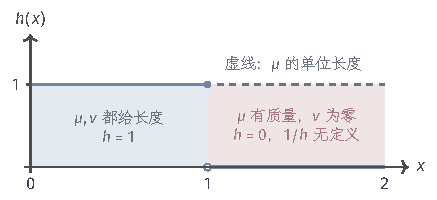
\includegraphics[width=73.914mm]{figures/02-abstract-mathematics/01-metric-and-measure/tikz/c4-one-sided-loss/figure.pdf}
  \caption{单向绝对连续时密度不能取倒数。参考测度$\mu$是$[0,2]$上的长度，目标测度$\nu$是$[0,1]$上的长度，密度$h=\mathbf 1_{[0,1]}$（蓝色实线）。在$[0,1]$上$h=1$，两种测度一致；在红色区域$(1,2]$上$h=0$，$\mu$有质量$1$而$\nu$没有质量，从$\nu$出发无法恢复这部分质量。}
  \label{fig:density-one-sided-loss}
\end{figure}
